\chapter{Cơ sở lý thuyết}
\label{Chapter2}
\section{Lý thuyết về học từ vựng và thuật toán lặp lại có khoảng cách}
Trong lĩnh vực tiếp thu ngôn ngữ thứ hai, từ vựng không chỉ là những đơn vị ngôn ngữ rời rạc mà còn là nền tảng cốt lõi chi phối khả năng vận hành cả bốn kỹ năng nghe, nói, đọc và viết \cite{Nation2001}. Tuy nhiên, thách thức lớn nhất đối với người học không nằm ở việc tiếp nhận thông tin mới, mà ở khả năng duy trì thông tin đó trong trí nhớ dài hạn. Thực tế này được làm sáng tỏ bởi Hermann Ebbinghaus thông qua khái niệm "đường cong quên lãng" (forgetting curve), mô tả sự suy giảm theo hàm mũ của dấu vết trí nhớ ngay sau khi quá trình học kết thúc \cite{Ebbinghaus1885}.
\begin{figure}[H]
\centering
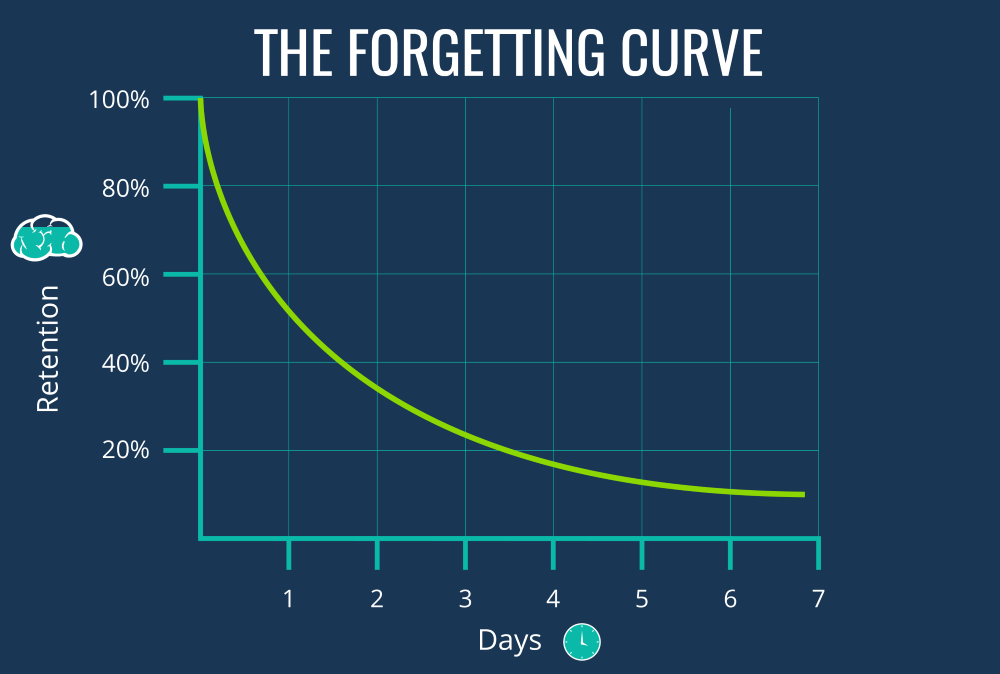
\includegraphics[width=13cm]{images/the-forgetting-curve.png}
\caption{Đường cong quên lãng.}
\label{fig_forgetting_curve}
\end{figure}
Quy luật tự nhiên này chỉ ra rằng nếu không có sự can thiệp kịp thời, phần lớn kiến thức sẽ biến mất chỉ sau một thời gian ngắn. Để đối phó với hiện tượng quên lãng, kỹ thuật lặp lại có khoảng cách (Spaced Repetition - SRS) đã ra đời như một giải pháp dựa trên bằng chứng khoa học \cite{Cepeda2008}. Thay vì nhồi nhét thông tin trong một thời gian ngắn, SRS tập trung vào việc dàn trải các phiên ôn tập theo thời gian. Nguyên lý then chốt của kỹ thuật này là thực hiện truy hồi thông tin ngay tại thời điểm trí nhớ bắt đầu suy giảm. Mỗi lần truy hồi thành công tại "điểm nút" này không chỉ khôi phục trí nhớ mà còn làm chậm đáng kể tốc độ quên lãng sau đó, giúp củng cố thông tin từ trí nhớ ngắn hạn sang trí nhớ dài hạn một cách bền vững \cite{Karpicke2008}.

Hiệu quả của mô hình SRS trong hệ thống này được hiện thực hóa thông qua thuật toán SM-2 (SuperMemo-2). Đây là một mô hình toán học cho phép cá nhân hóa hoàn toàn lộ trình học tập dựa trên khả năng phản hồi của từng cá nhân. Khác với các cơ chế nhắc nhở cố định, SM-2 vận hành dựa trên sự biến thiên của chỉ số độ dễ (Easiness Factor - EF) — đại lượng đại diện cho độ phức tạp của một từ vựng đối với một người học cụ thể. Thông qua điểm số chất lượng phản hồi ($q$) từ 0 đến 5, hệ thống sẽ liên tục điều chỉnh $EF$ theo công thức:

$$EF' = EF + (0.1 - (5 - q) \times (0.08 + (5 - q) \times 0.02))$$

Dựa trên chỉ số này, khoảng cách giữa các lần ôn tập ($I$) sẽ được mở rộng dần theo cấp số nhân. Trong đó, lần ôn tập thứ nhất ($I_1$) thường là sau 1 ngày, lần thứ hai ($I_2$) là 6 ngày, và từ lần thứ $n$ trở đi, khoảng cách được tính theo công thức $I_n = I_{n-1} \times EF$. Một đặc điểm quan trọng của thuật toán là việc duy trì ngưỡng $EF \ge 1.3$ — giá trị này không bao giờ được phép rơi dưới mức này, ngay cả khi người học trả lời sai nhiều lần. Ràng buộc này đảm bảo rằng ngay cả những từ vựng khó nhất vẫn được ôn tập với tần suất hợp lý, tránh việc khoảng cách ôn tập bị nén quá mức — điều dễ dẫn đến cảm giác nhàm chán và ảnh hưởng tiêu cực đến động lực học tập dài hạn.

Sự linh hoạt của SM-2 nằm ở cơ chế "thử thách vừa đủ": nếu người học trả lời sai ($q < 3$), thuật toán sẽ lập tức thiết lập lại chu kỳ về 0, buộc từ vựng đó phải xuất hiện thường xuyên hơn để củng cố lại dấu vết trí nhớ. Ngược lại, những từ vựng dễ sẽ được đẩy xa hơn trong lịch trình, giúp tối ưu hóa thời gian và công sức. Sự kết hợp giữa quy luật tâm lý học của Ebbinghaus và tính chính xác của thuật toán SM-2 tạo nên một động lực học tập dựa trên sự tiến bộ thực tế, đặt nền móng cho việc xây dựng thói quen ghi nhớ bền vững trong hệ thống.


\section{Lý thuyết Gamification và Cơ chế Thúc đẩy Động lực}

Mặc dù các giải pháp kỹ thuật như SM-2 đã tối ưu hóa được lộ trình ghi nhớ, thách thức lớn nhất vẫn nằm ở việc duy trì sự kiên trì của người học trước những rào cản về mặt tâm lý. Để giải quyết vấn đề này, Gamification được tích hợp nhằm bổ sung cơ chế trò chơi vào quy trình học tập để duy trì sự tham gia của người dùng \cite{Deterding2011}. Bằng cách lồng ghép các yếu tố đặc trưng của trò chơi, hệ thống hỗ trợ quá trình nội tâm hóa động lực học tập theo phổ của SDT \cite{Hamari2014}. Nhằm hạn chế các tác động tiêu cực của áp lực thành tích, hệ thống vận dụng khung lý thuyết Thuyết Tự Quyết (Self-Determination Theory - SDT) làm cơ sở thiết kế \cite{RyanDeci2017}.

Cốt lõi của SDT nhấn mạnh rằng động lực bền vững được hình thành khi các nhu cầu tâm lý cơ bản được đáp ứng. Trong đó, cảm giác về \textbf{Sự thành thạo (Competence)} được củng cố thông qua hệ thống phản hồi. Điểm tích lũy và hệ thống thăng cấp được thiết kế để phản ánh tiến trình phát triển năng lực, giúp người học nhận diện sự tiến bộ và duy trì động lực.

Tính \textbf{Tự quyết (Autonomy)} trong hệ thống được thể hiện qua quyền tự do xây dựng kho học liệu. Thay vì tuân theo một khuôn mẫu cố định, người dùng được chủ động biên soạn kho từ vựng cá nhân và lựa chọn thú ảo \cite{WerbachHunter2012}. Sự tự chủ này giúp người học chủ động hơn trong việc xây dựng lộ trình học tập theo nhu cầu cá nhân. Đồng thời, nhu cầu về \textbf{Sự kết nối (Relatedness)} được đáp ứng qua môi trường tương tác cộng đồng. Các bảng xếp hạng không chỉ khích lệ cạnh tranh mà còn tạo ra môi trường tương tác xã hội, qua đó đáp ứng nhu cầu gắn kết theo SDT.

Đặc điểm thiết kế trọng tâm của Gamification trong hệ thống là cơ chế thú ảo: khác với mô hình đặt streak (chuỗi ngày học liên tục) làm cơ chế gắn kết chủ đạo --- nơi một ngày bỏ học là thất bại hoàn toàn --- hệ thống xác định sự tăng trưởng của thú ảo là trục động lực trung tâm. Streak vẫn được ghi nhận như một chỉ số bổ sung về tính kỷ luật, nhưng điểm khác biệt then chốt là XP tích lũy cho thú ảo không bao giờ mất đi dù người học gián đoạn --- sự tiến hóa diễn ra theo quy luật tích lũy thuần túy, không có hình phạt hồi quy. Việc chuyển hóa nỗ lực học tập thành sự phát triển của thú ảo giúp giảm bớt áp lực tâm lý, thúc đẩy sự gắn kết với quá trình học tập. Cần lưu ý rằng, theo phổ liên tục của SDT \cite{RyanDeci2017}, phần thưởng ngẫu nhiên (cơ chế xác suất bắt thú) thuộc nhóm điều tiết ngoại tại, trong khi sự tiến hóa theo XP tích lũy --- gắn trực tiếp với nỗ lực học thuật --- hướng tới nhóm điều tiết đã được nội tâm hóa, tức người học tự nhận thấy giá trị của hoạt động. Sự kết hợp giữa hai mức độ điều tiết này nhằm hỗ trợ quá trình chuyển hóa từ động lực bên ngoài sang động lực bên trong theo phổ SDT.

\section{Vai trò của sự đối kháng và cạnh tranh}

Trong cấu trúc của hệ thống, chế độ chiến đấu (Battle Mode) không đơn thuần được thiết kế như một tính năng giải trí bề nổi, mà là ứng dụng có chủ đích của các nguyên lý khoa học giáo dục nhằm hỗ trợ quá trình tiếp thu ngôn ngữ.

Luận điểm đầu tiên nằm ở việc vận dụng Thuyết Xung đột Nhận thức (Cognitive Conflict Theory) \cite{Limon2001} kết hợp với khái niệm "Khó khăn thử thách có chủ đích" (Desirable Difficulties) \cite{Bjork2011}. Trong các trận đấu PvP/PvE, người học phải đồng thời xử lý kiến thức từ vựng và ra quyết định chiến thuật — chẳng hạn lựa chọn hệ thú theo nguyên tắc khắc chế (Lửa khắc Cỏ, Cỏ khắc Nước, Nước khắc Lửa) — trong khoảng thời gian hạn chế. Áp lực kép này buộc não bộ phải truy hồi từ vựng có chủ đích dưới điều kiện cạnh tranh, hiện thực hóa đúng bản chất của thực hành truy hồi chủ động. Nghiên cứu của Karpicke và Roediger \cite{Karpicke2008} chỉ ra rằng việc truy xuất thông tin dưới áp lực thời gian mang lại hiệu quả ghi nhớ dài hạn vượt trội so với học tập thụ động, kết quả được Carpenter \cite{Carpenter2012} xác nhận thêm trong bối cảnh học ngôn ngữ.


Bên cạnh đó, hệ thống tận dụng Thuyết Gắn kết Xã hội (Social Interdependence Theory) \cite{Johnson2009} để chuyển hóa các tương tác cạnh tranh thành động lực tự thân. Thông qua các bảng xếp hạng công khai và đấu trường trực tuyến, việc học không còn là một quá trình đơn độc mà gắn liền với vị thế xã hội trong một cộng đồng ảo. Theo SDT của Ryan và Deci \cite{RyanDeci2017}, sự cạnh tranh lành mạnh này thỏa mãn nhu cầu về năng lực (competence) và sự gắn kết (relatedness), từ đó thúc đẩy người học duy trì kỷ luật học tập một cách tự nguyện và bền bỉ hơn. Các nghiên cứu thực nghiệm của Hamari et al. \cite{Hamari2014} cũng chỉ ra rằng các yếu tố trò chơi hóa (gamification) có tác động tích cực đến thái độ và hành vi của người dùng khi được thiết kế đúng cách \cite{Deterding2011}.

Cuối cùng, sự đối kháng được tinh chỉnh để đưa người học vào Trạng thái Dòng chảy (Flow State) \cite{Csikszentmihalyi1990} thông qua hệ thống Gym Leader với độ khó tăng dần. Việc cân bằng giữa kỹ năng hiện tại của người học và thử thách của trò chơi là yếu tố then chốt để duy trì sự tập trung cực độ, tránh gây ra cảm giác nhàm chán hoặc lo âu quá mức \cite{WerbachHunter2012}. Cơ chế này biến việc truy hồi từ vựng thành yếu tố quyết định kết quả trận đấu, tạo động cơ ôn tập cụ thể. Cách tiếp cận này không chỉ nâng cao hiệu quả sư phạm mà còn hiện thực hóa mô hình học tập chủ động \cite{Prince2004}, giúp người học làm chủ kiến thức thông qua quá trình vận dụng trực tiếp vào các tình huống thực tế trong hệ thống \cite{Nation2001}.
\section{Các công trình và ứng dụng liên quan}

Việc ứng dụng các lý thuyết khoa học nhận thức như lặp lại ngắt quãng và thực hành truy hồi vào giáo dục ngôn ngữ đã được minh chứng qua sự thành công của nhiều nền tảng số. Tuy nhiên, qua quá trình khảo sát và phân tích các ứng dụng tiêu biểu, kết quả cho thấy vẫn tồn tại những rào cản nhất định trong việc cân bằng giữa hiệu quả học thuật và sự gắn kết cảm xúc bền vững.

Điển hình là trường hợp của \textbf{Duolingo}, nền tảng dẫn đầu về việc vận dụng các chỉ số định lượng như điểm kinh nghiệm (XP), bảng xếp hạng và chuỗi ngày học tập (streak) để duy trì thói quen người dùng. Mặc dù phương thức này tạo ra động lực tiếp cận ban đầu rất tốt, nhưng dưới góc độ tâm lý học hành vi, việc quá chú trọng vào các chỉ số ngoại tại dễ dẫn đến trạng thái áp lực tinh thần. Hệ quả là khi chuỗi ngày học tập bị đứt quãng, người học thường rơi vào trạng thái kiệt sức học tập và có xu hướng từ bỏ lộ trình thay vì tái kết nối \cite{DuolingoBlog2024}. Đây chính là \textbf{khoảng trống về tính bền vững của động lực}: hệ thống đang ưu tiên việc duy trì con số hơn là xây dựng một sợi dây liên kết nội tại giữa người học và tiến trình phát triển cá nhân.

Trong khi đó, \textbf{Quizlet} lại tiếp cận theo hướng đề cao quyền tự chủ, cho phép cá nhân hóa tối đa kho học liệu thông qua các bộ flashcard tự tạo \cite{QuizletLearn2024}. Tuy nhiên, điểm yếu cố hữu của mô hình này là sự vắng bóng của các cơ chế Gamification chuyên sâu, khiến nó dừng lại ở mức một công cụ hỗ trợ thuần túy. Sự thiếu hụt trong việc thỏa mãn đồng bộ ba nhu cầu cơ bản của thuyết Tự quyết (SDT) — bao gồm năng lực, tự chủ và sự gắn kết — dẫn đến việc người học cần một tinh thần tự giác cực cao để không bỏ dở giữa chừng.

Ở một thái cực khác, các công cụ như \textbf{Anki} và \textbf{Memrise} lại tập trung tối đa vào tính chính xác của thuật toán SRS để tối ưu hóa khả năng ghi nhớ dài hạn \cite{AnkiWeb2024, MemriseHelp2024}. Dù đạt hiệu quả cao về mặt kỹ thuật, nhóm ứng dụng này thường gặp rào cản lớn về trải nghiệm người dùng (UX) do giao diện khô khan và thiếu đi tính tương tác xã hội. Việc thiếu vắng yếu tố tự sự (narrative) và cơ chế phản hồi thiếu đa dạng khiến quy trình học tập trở nên đơn điệu, thiếu phản hồi tích cực.

Nhận diện khoảng trống nói trên, hệ thống được xây dựng nhằm tạo ra môi trường học tập nơi thuật toán SRS vận hành gắn liền với tiến trình phát triển của thú ảo, để mỗi từ vựng được ghi nhớ đóng góp trực tiếp vào sự phát triển đó.

Từ việc phân tích trên, có thể tổng kết \textbf{ba khoảng trống nghiên cứu (Research Gaps)} chính mà các hệ thống hiện tại chưa giải quyết triệt để:

\begin{itemize}
\item \textbf{Thiếu cơ chế gắn kết tích lũy bền vững:} Các hệ thống hiện có đặt streak (chuỗi ngày học liên tục) làm cơ chế gắn kết chủ đạo, khiến sự gián đoạn học tập --- điều không thể tránh trong thực tế --- trở thành tác nhân trực tiếp phá vỡ động lực. Khoảng trống này là cơ sở để thiết kế hệ thống với trục gắn kết dựa trên tích lũy XP không hồi quy (pet XP không bao giờ bị mất), kết hợp với hệ thống nhiệm vụ hàng ngày tạo các mốc ngắn hạn, thay vì phụ thuộc vào mô hình streak thuần túy.
\item \textbf{Sự mất cân bằng trong Gamification:} Phần lớn ứng dụng chỉ tập trung vào một vài yếu tố bề nổi (XP, Leaderboard, Streak) mà chưa triển khai hài hòa cả ba nhu cầu tâm lý cơ bản của Thuyết Tự Quyết (SDT): năng lực (competence), tự chủ (autonomy) và gắn kết (relatedness). Đặc biệt, tính tự chủ trong hầu hết các ứng dụng bị thu hẹp trong phạm vi lựa chọn nội dung, chứ chưa mở rộng sang quyền định hình hành trình học tập theo cách có ý nghĩa cá nhân.
\item \textbf{Sự thiếu hụt mô hình tích hợp SRS và Gamification:} Trong phạm vi các ứng dụng được khảo sát, chưa tìm thấy hệ thống nào tích hợp đồng thời: thuật toán SRS theo chuẩn SM-2, cơ chế Gamification gắn với thú ảo theo mô hình SDT, và tích lũy tiến trình không hồi quy. Nhận định này dựa trên phân tích tính năng công khai của các ứng dụng; so sánh có kiểm chứng là hướng nghiên cứu cần tiếp nối.
\end{itemize}

Đây chính là điểm cốt lõi mà hệ thống hướng tới: xây dựng cơ chế tích lũy có phản hồi trực quan, trong đó tiến trình học tập gắn liền trực tiếp với sự phát triển của thú ảo nhằm cụ thể hóa nhu cầu về năng lực (Competence) theo SDT.

\section{Hệ sinh thái công nghệ triển khai}

Để hiện thực hóa các mục tiêu về trải nghiệm tương tác tức thời và đảm bảo tính ổn định lâu dài cho hệ thống, việc lựa chọn nền tảng kỹ thuật được cân nhắc dựa trên sự giao thoa giữa hiệu năng vận hành và khả năng bảo trì mã nguồn. Cấu trúc công nghệ cốt lõi của dự án được định hình bởi bộ ba: ASP.NET Core điều phối logic tại tầng Backend, ReactJS (kết hợp cùng Vite và TypeScript) đảm nhiệm giao diện Frontend, và SQL Server chịu trách nhiệm quản trị dữ liệu quan hệ. Sự hội tụ của những công nghệ này cung cấp nền tảng kỹ thuật cho việc triển khai các tính năng đã đề ra và mở rộng trong các giai đoạn tiếp theo.

\subsection{Nền tảng Backend: ASP.NET Core}

Việc tin dùng ASP.NET Core làm "xương sống" cho tầng xử lý trung tâm xuất phát từ nhu cầu về một hệ thống có tính kỷ luật cao và hiệu suất thực thi mạnh mẽ. Cơ chế kiểm soát kiểu dữ liệu tĩnh của C\# giúp phát hiện sai sót tại giai đoạn biên dịch, hỗ trợ tái cấu trúc mã nguồn với độ an toàn cao hơn so với các ngôn ngữ kiểm soát kiểu động \cite{MicrosoftASPNETCore2024}. Đối với các tác vụ như tính toán lịch trình SRS và xử lý dữ liệu thời gian thực, framework vận hành hiệu quả nhờ mô hình bất đồng bộ tích hợp sẵn.

Các thành phần nội tại của framework được vận dụng cụ thể như sau. Cụ thể, máy chủ web Kestrel được triển khai để xử lý lưu lượng cao, hỗ trợ các kết nối WebSocket cần thiết cho việc cập nhật điểm số và kết quả quiz theo thời gian thực \cite{KestrelDocs2024}. Kiến trúc Middleware được thiết kế theo dạng chuỗi nối tiếp, giúp tách biệt các lớp bảo mật JWT và xử lý ngoại lệ tập trung \cite{MiddlewareDocs2024}. Thêm vào đó, việc áp dụng mẫu thiết kế Dependency Injection tích hợp sẵn đã giúp chuẩn hóa mô hình Controller–Service–Repository, không chỉ nâng cao tính độc lập của các module để phục vụ kiểm thử mà còn giảm bớt rủi ro khi thay đổi logic nghiệp vụ. Lập trình bất đồng bộ (Async/Await) và Entity Framework Core hỗ trợ quản trị tài nguyên máy chủ và điều chỉnh lược đồ dữ liệu qua migrations \cite{MicrosoftEFCore2024}.

\subsection{Lớp giao diện tương tác: ReactJS}

Trong vai trò là cầu nối trực tiếp với người dùng, ReactJS được lựa chọn nhờ khả năng xây dựng giao diện tương tác với tốc độ phản hồi cao. Do đặc thù của dự án yêu cầu sự đồng bộ liên tục giữa tiến độ học và trạng thái sinh trưởng của thú ảo, cơ chế Virtual DOM của ReactJS phù hợp để xử lý các cập nhật giao diện phức tạp với hiệu suất ổn định \cite{ReactDocs2024}. Triết lý thiết kế dựa trên thành phần (Component-based) cho phép phân rã giao diện thành những khối chức năng độc lập, giúp việc tái sử dụng mã nguồn trở nên dễ dàng và đảm bảo sự đồng nhất về mặt thẩm mỹ cho toàn bộ ứng dụng UI trong dài hạn.

Khả năng duy trì sự ổn định cho các màn hình có mật độ tương tác dày đặc được đảm bảo bởi thuật toán Reconciliation, giúp tiết giảm tối đa các thao tác can thiệp trực tiếp vào DOM thực \cite{ReactVirtualDOM2024}. Việc quản lý trạng thái và các tác vụ ngoại vi (side-effects) được thực hiện một cách tường minh thông qua React Hooks, kết hợp cùng TypeScript để tạo ra một "màng lọc" lỗi kiểu dữ liệu ngay từ đầu. Để bứt phá về tốc độ phát triển, dự án tích hợp Vite như một công cụ đóng gói thế hệ mới, mang lại trải nghiệm lập trình mượt mà với tính năng thay đổi nóng (HMR) tức thì \cite{ViteDocs2024}. Tailwind CSS theo hướng utility-first được áp dụng để xây dựng giao diện đồng nhất và tương thích đa kích thước màn hình.

\subsection{Quản trị dữ liệu: SQL Server}

SQL Server được chọn nhờ sự tương thích tốt trong hệ sinh thái .NET và hỗ trợ tiêu chuẩn ACID đảm bảo tính nhất quán dữ liệu \cite{SQLServerDocs2024}. Trong bối cảnh giáo dục, tính toàn vẹn của dữ liệu lịch sử học tập là yêu cầu quan trọng; SQL Server đáp ứng yêu cầu này cùng các công cụ giám sát tích hợp. Sự kết hợp giữa các kỹ thuật tối ưu truy vấn hiện đại như Columnstore Index và khả năng vận hành linh hoạt trên môi trường đám mây giúp hệ thống đạt được sự cân bằng giữa tốc độ truy xuất và khả năng mở rộng quy mô.

\subsection{Các dịch vụ tích hợp đám mây}

Bên cạnh bộ ba nền tảng cốt lõi, hệ thống tích hợp một lớp dịch vụ đám mây chuyên biệt nhằm tự động hóa các tác vụ đòi hỏi năng lực xử lý vượt ra ngoài khả năng của một ứng dụng đơn lẻ.

\textbf{Google Gemini API} được tích hợp để sinh tự động các thuộc tính ngôn ngữ học của từ vựng, bao gồm phiên âm IPA, nghĩa tiếng Việt, câu ví dụ ngữ cảnh, từ loại và cấp độ CEFR tương ứng. Việc khai thác mô hình ngôn ngữ lớn (LLM) cho phép hệ thống cung cấp dữ liệu chất lượng cao mà không yêu cầu biên soạn thủ công, đồng thời cho phép mở rộng kho từ vựng mà không cần biên soạn thủ công.

\textbf{Azure AI Speech Services} cung cấp công nghệ tổng hợp giọng nói (Text-to-Speech) với giọng đọc chuẩn \texttt{en-US-AndrewNeural}, xuất tệp MP3 và lưu trữ trên Azure Blob Storage. Cơ sở hạ tầng CDN tích hợp của Azure đảm bảo tệp âm thanh được phân phối tới người dùng với độ trễ thấp, phục vụ trực tiếp cho loại câu hỏi nghe hiểu (Listening) trong các phiên học.

\textbf{Redis} đóng vai trò là lớp bộ nhớ đệm phân tán (Distributed Cache) thông qua giao diện \texttt{IDistributedCache} của ASP.NET Core. Kết quả sinh metadata từ Gemini API được lưu vào bộ nhớ đệm với thời gian tồn tại 7 ngày, giúp loại bỏ các lần gọi API trùng lặp và giảm đáng kể chi phí vận hành. Hệ thống được thiết kế theo nguyên tắc xuống cấp nhẹ nhàng (graceful degradation): khi Redis không khả dụng, luồng xử lý tiếp tục bình thường thông qua API trực tiếp mà không gây gián đoạn dịch vụ.

\subsection{Phân tích tổng hợp}

Kết hợp giữa ASP.NET Core, ReactJS và SQL Server tạo thành một khung kỹ thuật ổn định cho việc triển khai các tính năng đã đặt ra. Trong khi tầng Backend xử lý các nghiệp vụ logic và dữ liệu tập trung, tầng Frontend ưu tiên tính đáp ứng trong trải nghiệm người dùng \cite{TechEmpower2024}.



